
\definecolor{cgreen}{HTML}{5BAD72}
\definecolor{corange}{HTML}{E8863A}
\definecolor{cblue}{HTML}{4A90D9}

\newcommand{\cellsize}{0.48}

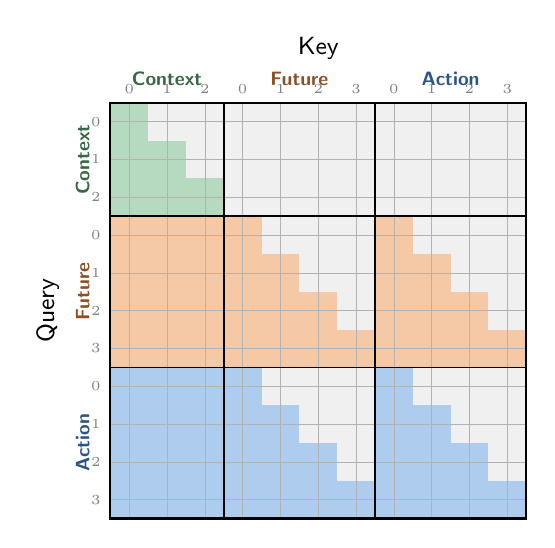
\begin{tikzpicture}[
    cell/.style={minimum size=\cellsize cm, inner sep=0pt, outer sep=0pt},
    attend/.style={cell, fill=#1!45},
    empty/.style={cell, fill=black!6},
    blklbl/.style={font=\tiny\sffamily\bfseries, rotate=90, anchor=south},
    blklblh/.style={font=\tiny\sffamily\bfseries, anchor=east},
]

% Grid dimensions: 3 context blocks + 4 future blocks + 4 action blocks = 11
\pgfmathsetmacro{\N}{11}
\pgfmathsetmacro{\Nm}{\N-1}

% Block ranges (0-indexed):
%   Context: 0,1,2        (C0, C1, C2)
%   Future:  3,4,5,6      (F0, F1, F2, F3)
%   Action:  7,8,9,10     (A0, A1, A2, A3)

% Draw all cells as empty first
\foreach \r in {0,...,\Nm} {
    \foreach \c in {0,...,\Nm} {
        \node[empty] at (\c*\cellsize, -\r*\cellsize) {};
    }
}

% --- Context rows: C_i attends to C_0..C_i ---
% C0 row
\foreach \c in {0} {
    \node[attend=cgreen] at (\c*\cellsize, 0) {};
}
% C1 row
\foreach \c in {0,1} {
    \node[attend=cgreen] at (\c*\cellsize, -1*\cellsize) {};
}
% C2 row
\foreach \c in {0,1,2} {
    \node[attend=cgreen] at (\c*\cellsize, -2*\cellsize) {};
}

% --- Future rows: F_i attends to all context + F_0..F_i + A_0..A_i ---
% F0: all C + F0 + A0
\foreach \c in {0,1,2, 3, 7} {
    \node[attend=corange] at (\c*\cellsize, -3*\cellsize) {};
}
% F1: all C + F0,F1 + A0,A1
\foreach \c in {0,1,2, 3,4, 7,8} {
    \node[attend=corange] at (\c*\cellsize, -4*\cellsize) {};
}
% F2: all C + F0..F2 + A0..A2
\foreach \c in {0,1,2, 3,4,5, 7,8,9} {
    \node[attend=corange] at (\c*\cellsize, -5*\cellsize) {};
}
% F3: all C + F0..F3 + A0..A3
\foreach \c in {0,1,2, 3,4,5,6, 7,8,9,10} {
    \node[attend=corange] at (\c*\cellsize, -6*\cellsize) {};
}

% --- Action rows: A_i attends to all context + F_0..F_i + A_0..A_i ---
% A0: all C + F0 + A0
\foreach \c in {0,1,2, 3, 7} {
    \node[attend=cblue] at (\c*\cellsize, -7*\cellsize) {};
}
% A1: all C + F0,F1 + A0,A1
\foreach \c in {0,1,2, 3,4, 7,8} {
    \node[attend=cblue] at (\c*\cellsize, -8*\cellsize) {};
}
% A2: all C + F0..F2 + A0..A2
\foreach \c in {0,1,2, 3,4,5, 7,8,9} {
    \node[attend=cblue] at (\c*\cellsize, -9*\cellsize) {};
}
% A3: all C + F0..F3 + A0..A3
\foreach \c in {0,1,2, 3,4,5,6, 7,8,9,10} {
    \node[attend=cblue] at (\c*\cellsize, -10*\cellsize) {};
}

% Grid lines
\draw[black!30, very thin] (-0.5*\cellsize, 0.5*\cellsize) grid[step=\cellsize] (\N*\cellsize - 0.5*\cellsize, -\N*\cellsize + 0.5*\cellsize);

% Section separators
\draw[black, semithick] (2.5*\cellsize, 0.5*\cellsize) -- (2.5*\cellsize, -\N*\cellsize + 0.5*\cellsize);
\draw[black, semithick] (6.5*\cellsize, 0.5*\cellsize) -- (6.5*\cellsize, -\N*\cellsize + 0.5*\cellsize);
\draw[black, semithick] (-0.5*\cellsize, -2.5*\cellsize) -- (\N*\cellsize - 0.5*\cellsize, -2.5*\cellsize);
\draw[black, semithick] (-0.5*\cellsize, -6.5*\cellsize) -- (\N*\cellsize - 0.5*\cellsize, -6.5*\cellsize);

% Outer border
\draw[black, thick] (-0.5*\cellsize, 0.5*\cellsize) rectangle (\N*\cellsize - 0.5*\cellsize, -\N*\cellsize + 0.5*\cellsize);

% Column labels (top)
\node[font=\scriptsize\sffamily\bfseries, text=cgreen!60!black, anchor=south] at (1*\cellsize, 0.7*\cellsize) {Context};
\node[font=\scriptsize\sffamily\bfseries, text=corange!60!black, anchor=south] at (4.5*\cellsize, 0.7*\cellsize) {Future};
\node[font=\scriptsize\sffamily\bfseries, text=cblue!60!black, anchor=south] at (8.5*\cellsize, 0.7*\cellsize) {Action};

% Row labels (left)
\node[font=\scriptsize\sffamily\bfseries, text=cgreen!60!black, rotate=90, anchor=south] at (-0.8*\cellsize, -1*\cellsize) {Context};
\node[font=\scriptsize\sffamily\bfseries, text=corange!60!black, rotate=90, anchor=south] at (-0.8*\cellsize, -4.5*\cellsize) {Future};
\node[font=\scriptsize\sffamily\bfseries, text=cblue!60!black, rotate=90, anchor=south] at (-0.8*\cellsize, -8.5*\cellsize) {Action};

% Block indices (top, small)
\foreach \i [evaluate=\i as \x using \i*\cellsize] in {0,1,2} {
    \node[font=\tiny\sffamily, text=black!50, anchor=south] at (\x, 0.5*\cellsize) {$\i$};
}
\foreach \i [evaluate=\i as \x using {(\i+3)*\cellsize}] in {0,1,2,3} {
    \node[font=\tiny\sffamily, text=black!50, anchor=south] at (\x, 0.5*\cellsize) {$\i$};
}
\foreach \i [evaluate=\i as \x using {(\i+7)*\cellsize}] in {0,1,2,3} {
    \node[font=\tiny\sffamily, text=black!50, anchor=south] at (\x, 0.5*\cellsize) {$\i$};
}

% Block indices (left, small)
\foreach \i [evaluate=\i as \y using {-\i*\cellsize}] in {0,1,2} {
    \node[font=\tiny\sffamily, text=black!50, anchor=east] at (-0.5*\cellsize, \y) {$\i$};
}
\foreach \i [evaluate=\i as \y using {-(\i+3)*\cellsize}] in {0,1,2,3} {
    \node[font=\tiny\sffamily, text=black!50, anchor=east] at (-0.5*\cellsize, \y) {$\i$};
}
\foreach \i [evaluate=\i as \y using {-(\i+7)*\cellsize}] in {0,1,2,3} {
    \node[font=\tiny\sffamily, text=black!50, anchor=east] at (-0.5*\cellsize, \y) {$\i$};
}

% Axis labels
\node[font=\small\sffamily, anchor=south] at ({(\N-1)*\cellsize/2}, 1.4*\cellsize) {Key};
\node[font=\small\sffamily, rotate=90, anchor=south] at (-1.6*\cellsize, {-(\N-1)*\cellsize/2}) {Query};

\end{tikzpicture}
